
This search~\cite{Khachatryan:2016kdk} looks for an anomalously high rate of events
with four or more jets,
no identified isolated electron or muon
or isolated charged track,
large $\Ht$, and large $\mht$.
The principal~\sm~backgrounds are
 events with top quarks,
W bosons and jets,
Z bosons and jets,
and QCD multi-jet production,
and are evaluated using control samples in the data as well 
as information based on simulated events.

The search targets simplified model scenarios corresponding to  
gluino pair production,
followed by the decay of each gluino to an LSP
and a b$\bar{\text{b}}$ pair (T1bbbb model),
to an LSP and a 
t$\bar{\text{t}}$ pair  (T1tttt model),
or to an LSP and  a light flavor q$\bar{\text{q}}$ pair (T1qqqq model).
Simplified models corresponding to gluino pair
production followed by the decay of each gluino to
a q$\bar{\text{q}}$ pair and
a next-to-lightest EWkino, $\tilde{\chi}^{0}_{2}$ or $\chi^{\pm}_{1}$ (T5qqqqVV model), 
are also targeted.
These models are shown in 
Fig. \ref{fig:Ra2bSMS}.
\begin{figure}[tb!]
\centering
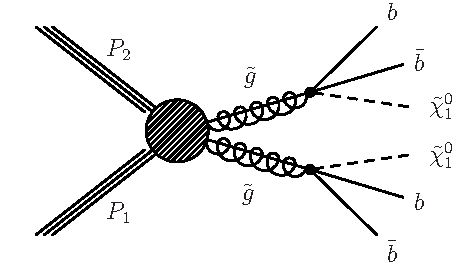
\includegraphics[width=0.45\textwidth]{figures/SusySearches/Ra2b2015/T1bbbb.pdf}
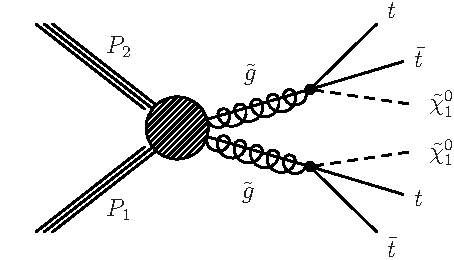
\includegraphics[width=0.45\textwidth]{figures/SusySearches/Ra2b2015/T1tttt.pdf}\\
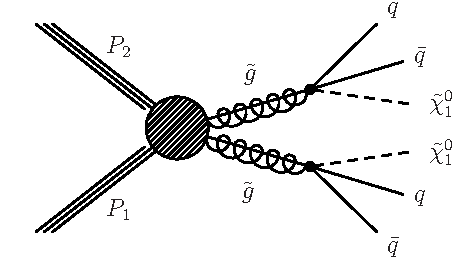
\includegraphics[width=0.45\textwidth]{figures/SusySearches/Ra2b2015/T1qqqq.pdf}
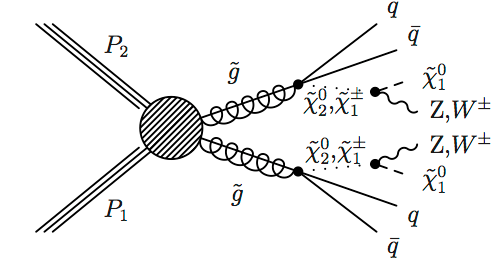
\includegraphics[width=0.45\textwidth]{figures/SusySearches/Ra2b2015/T5vv.pdf}
\caption{
  The simplified models used for the optimization and interpretation of the multi-jet $+$ $\mht$ search. 
  They are T1bbbb (upper left), T1tttt (upper right), T1qqqq (lower left), and T5qqqqVV (lower right) scenarios.
}
\label{fig:Ra2bSMS}
\end{figure}

Events are collected using the hadronic trigger named
\begin{itemize}
  \item \texttt{HLT\_PFHT350\_PFMET100\_*},
\end{itemize}
where the text PFHT and PFMET refer to the online $\Ht$ and $\met$ computed using the particle flow (PF) algorithm (Section \ref{sec:reconstruction}), and the numbers 350 and 100 refer to the respective triggering thresholds in units of GeV.

At level 1 of the trigger system, events are triggered if they have a calorimeter-based $\Ht$ of 175 GeV. If the event is accepted, the HLT trigger then requires a calorimeter-based $\Ht>$ 280 GeV and a calorimeter-based $\met>$ 70 GeV. Finally, the HLT trigger applies a lower threshold of 350 GeV on the $\Ht$ in coincidence with a threshold on the $\met$ above 100 GeV computed using all particles reconstructed from information from the tracker and calorimeters.

\begin{figure}[tb!]
  \begin{center}
    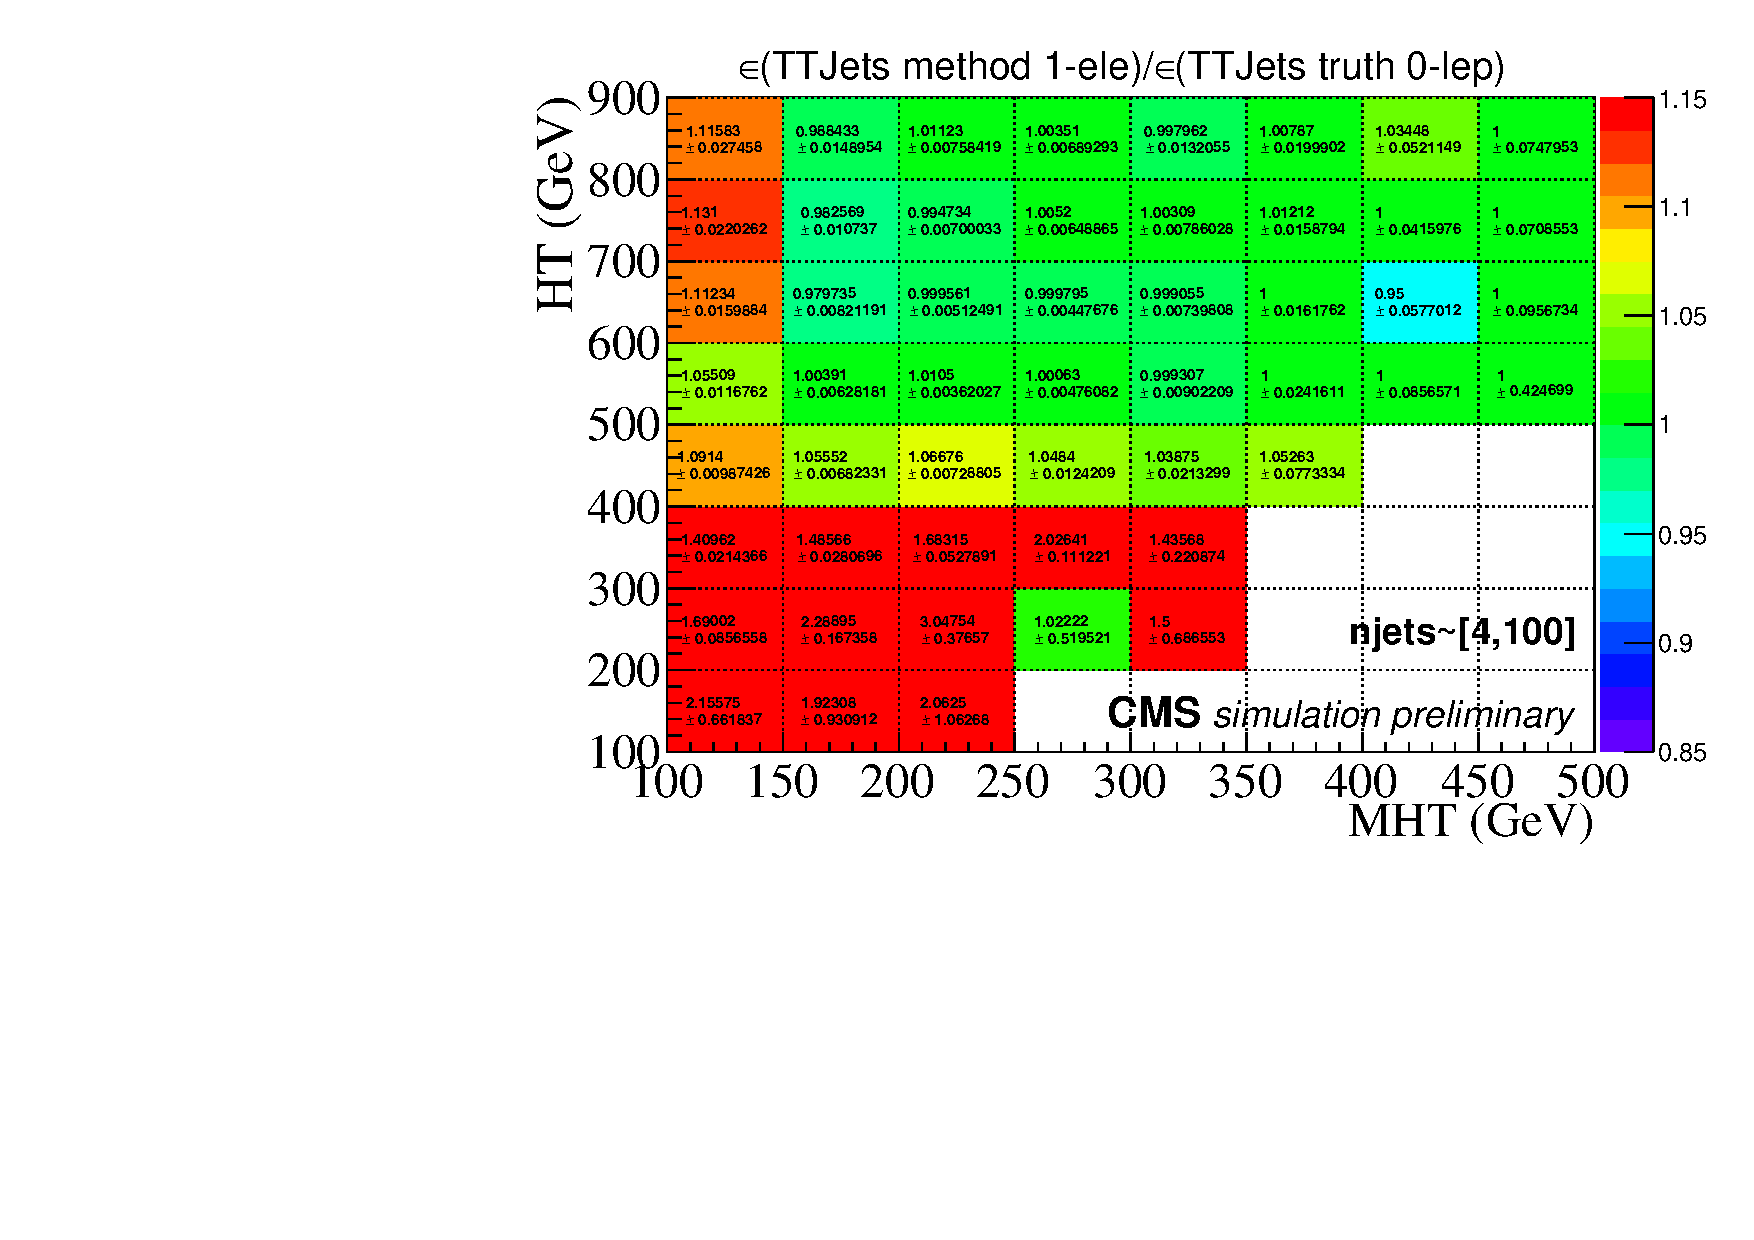
\includegraphics[width=0.95\linewidth]{figures/trigger/EfficiencyRatioMethodTruth.pdf}
    \caption{
      The ratio of the trigger efficiency for events passing the single
      electron reference trigger to the trigger efficiency for all
      events in a simulated t$\bar{\text{t}}$ sample, as a function of the offline $\Ht$
      and $\mht$. The ratio is consistent with 1 within the region of
      the baseline selection of $\Ht>500$ GeV and $\mht>200$ GeV of the CMS hadronic searches.
    }
    \label{fig:2dEffRatio}
  \end{center}
\end{figure}
It is seen that this choice of reference trigger allows for an unbiased estimate of the trigger efficiency in the region $\mht>150$ GeV and $\Ht>500$, which fortunately includes the baseline selection of the analyses that use this trigger; the baseline region definitions impose offline selections of $\mht>200$ GeV and $\Ht>500$ GeV, indicated below. 

The efficiency, estimated without bias using Equation \ref{eq:trigeff}, is shown as a function of the offline $\Ht$ and $\mht$, each in 1-dimension, in Fig. \ref{fig:trigger-turnon} using the entire 2015 dataset. 
\begin{figure}[tb!]
  \begin{center}
    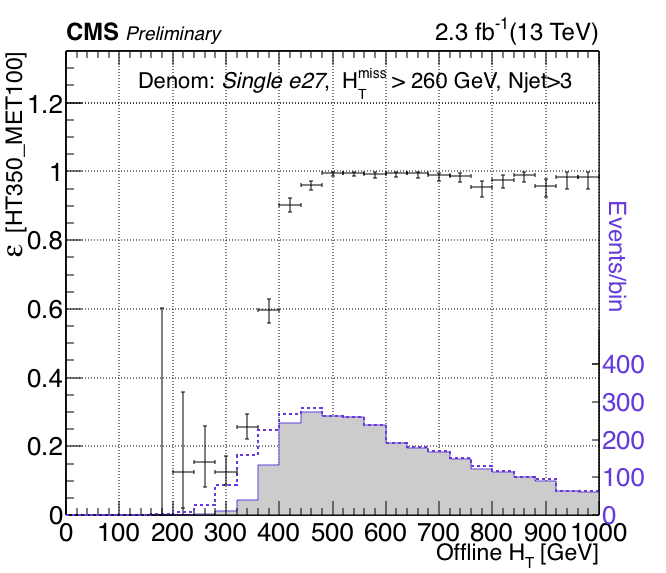
\includegraphics[width=0.49\linewidth]{figures/trigger/EffVsHt2_3InvFb.png}
    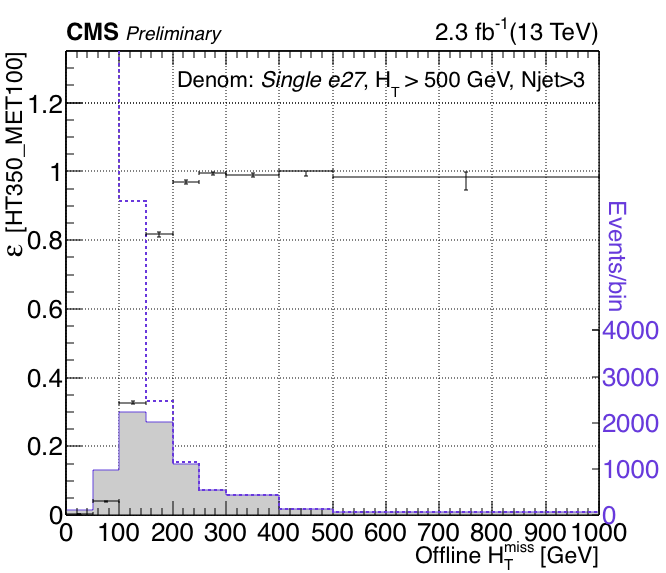
\includegraphics[width=0.49\linewidth]{figures/trigger/EffVsMht2_3InvFb.png}
    \caption{
      The trigger efficiency for \texttt{HLT\_PFHT350\_PFMET100*} 
      as a function of the search variables $\Ht$ and $\mht$. The dashed (solid) blue
      lines show the distributions of the denominator (numerator) samples. These results were used in the CMS PAS on the commissioning of 13 TeV observables for SUSY searches~\cite{CMS-DP-2015-035}.
      }
    \label{fig:trigger-turnon}
  \end{center}
\end{figure}
The statistical uncertainties in the plot are the 68\% CL Clopper-Pearson
intervals~\cite{Clopper:Pearson}. Additionally, a systematic uncertainty is assigned to the efficiency
equal to the difference between the efficiency obtained from applying the method described to a
sample of simulated t$\bar{\text{t}}$ events and that derived
from a set of simulated signal events. Such differences may arise due to any number of subtle differences in the content of the events in t$\bar{\text{t}}$ and signal samples. 

The probability for the trigger to fire on an event that passes the baseline selection is greater than 97\%. The baseline event selection can be summarized as follows. Events are accepted if they have
\begin{itemize}
\item no reconstructed, isolated lepton with a $\pt>10$ GeV and $|\eta|<2.4$, where the isolation is as defined in Equation \ref{eq:isolation};
\item no reconstructed, isolated particle track with a $\pt>10$ GeV and $|\eta|<2.4$;
\item $\Ht>500$ GeV;
\item $\mht>200$ GeV;
\item $\njets\geq$ 4, where jets are required to have a $\pt>30$ GeV and $|\eta|<2.4$, and
\item $\Delta\phi(\mht$, jet$_{1,2,3,4})>$ 0.5, 0.5, 0.3, 0.3.
\end{itemize}
After this selection, events are further subdivided into 72 exclusive bins
in a four-dimensional array of $\mht$,
the number of jets,
the number of tagged bottom quark jets,
and $\Ht$. Figure \ref{fig:ra2bArray} shows the boundaries of 6 bins in the $\Ht-\mht$ plane, and 12 bins in the plane of $\njets$$-$$\nbjets$. The 72 bins included in this search are defined by each unique combination of a box in the $\mht$$-$$\Ht$ plane and a box in the $\njets$$-$$\nbjets$ plane. 
\begin{figure}[tb!]
\centering
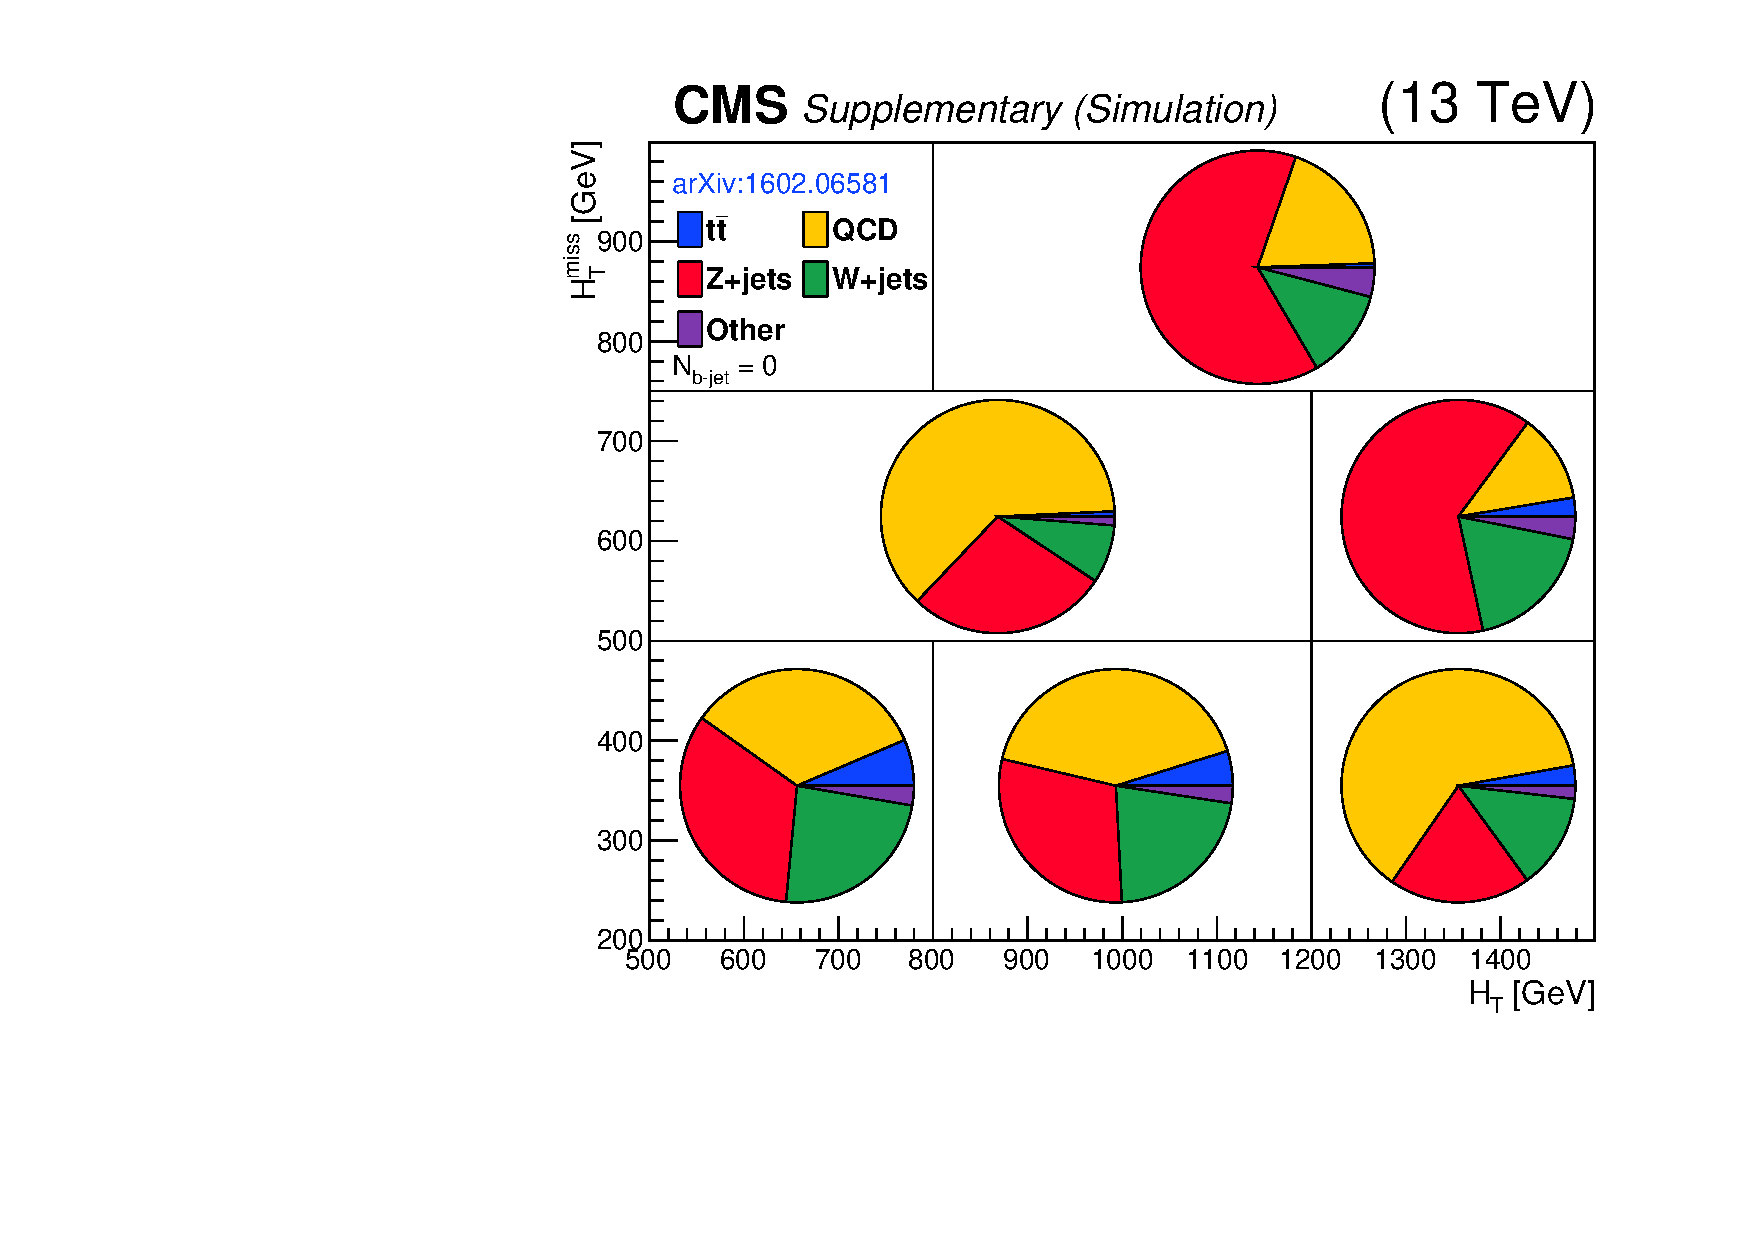
\includegraphics[height=0.442\textwidth]{figures/SusySearches/Ra2b2015/aux/MC_BG_Pie_NB0.pdf}
\hspace{-1cm}
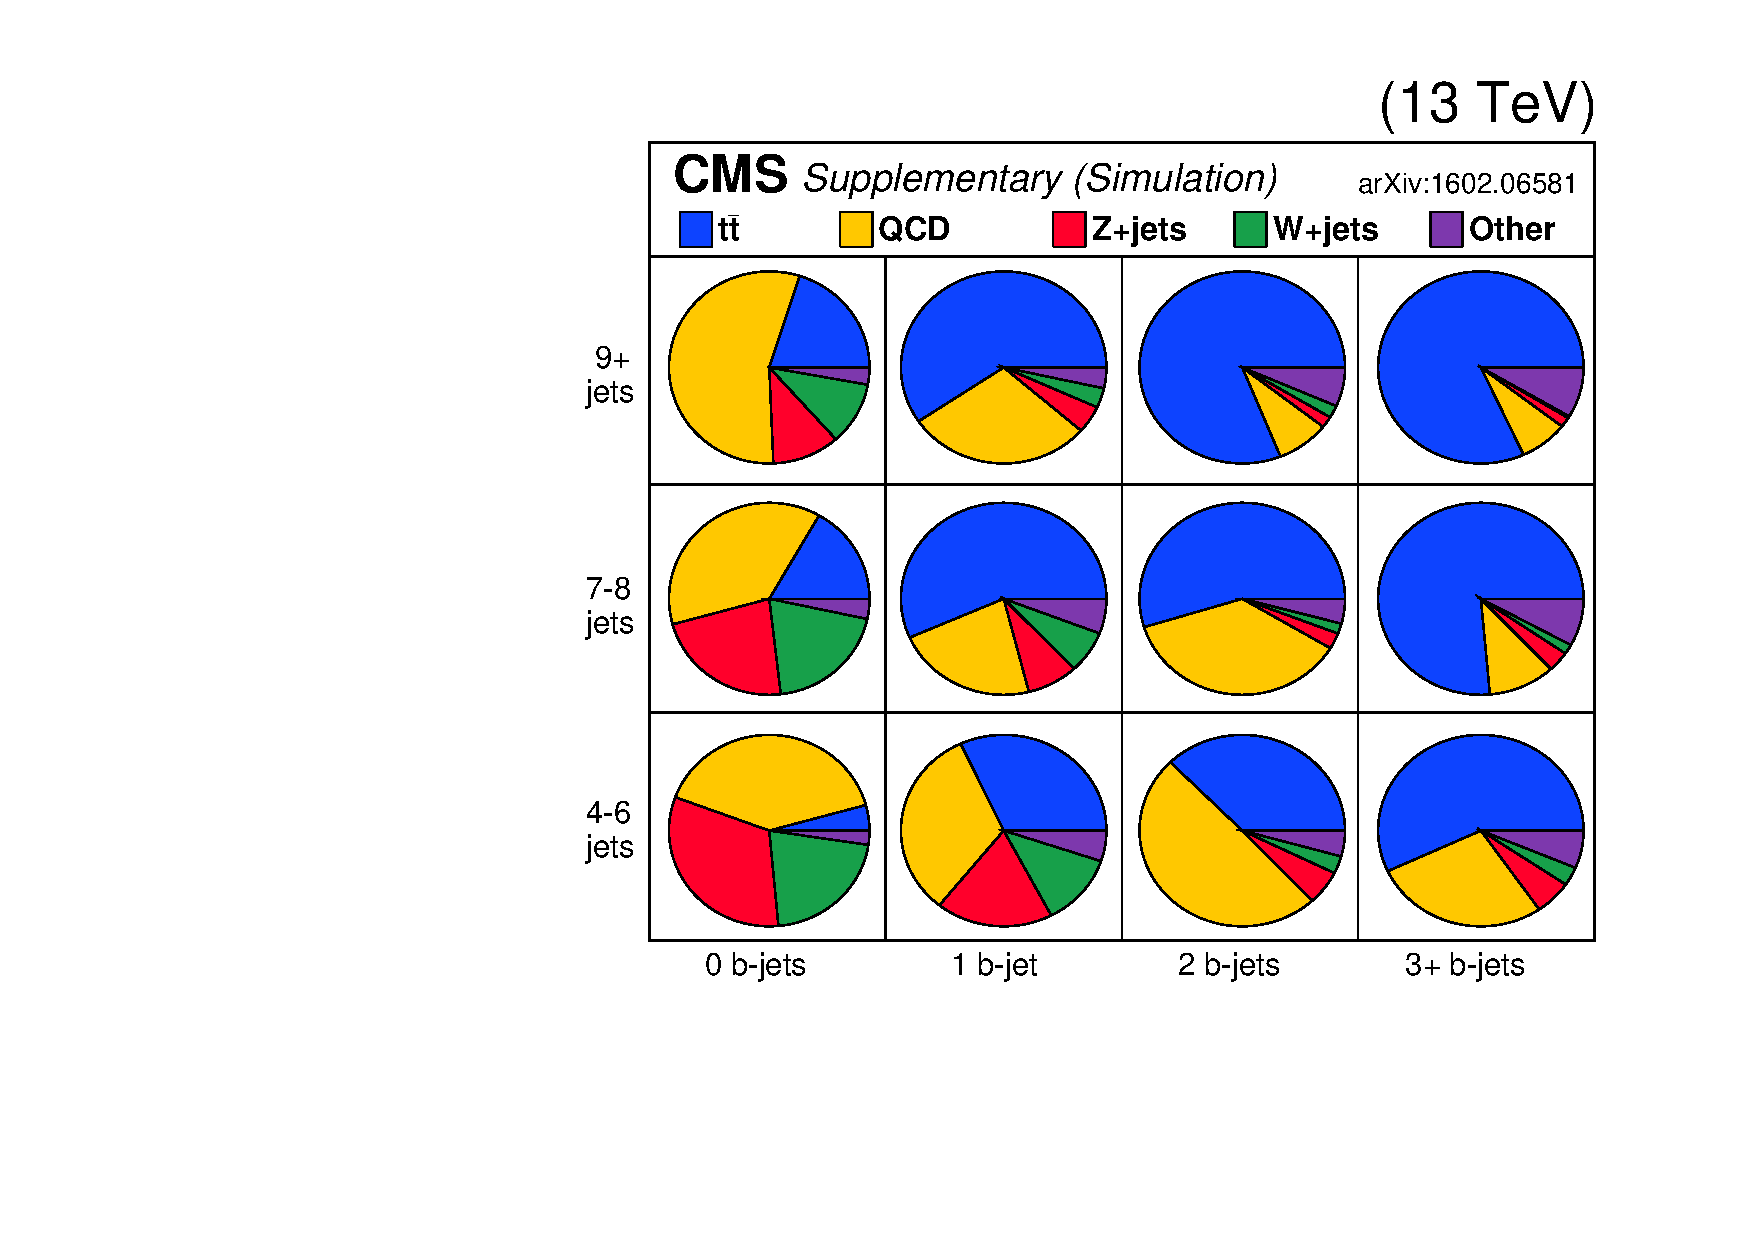
\includegraphics[height=0.445\textwidth]{figures/SusySearches/Ra2b2015/aux/MC_BG_Pie_vs_NJets_NBJets.pdf}
\caption{The signal region boundaries in the planes of $\mht$$-$$\Ht$ (top) and $\njets$$-$$\nbjets$ (bottom) for the multi-jet $+$ $\mht$ 
search. The pie charts represent the relative contributions
 to the~\sm~backgrounds in the region $\njets=$ 4$-$6, $\nbjets=0$ (top), and $\mht=$ 200$-$500 GeV, $\Ht=$ 500$-$750 GeV (bottom).}
\label{fig:ra2bArray}
\end{figure}


\subsubsection{Background estimation}
The relative contribution of each~\sm~background in the selected regions is also shown in Fig. \ref{fig:ra2bArray}. The t$\bar{\text{t}}$, W$+$jets, and Z$+$jets backgrounds are estimated by data-driven methods are detailed in  \cite{Khachatryan:2016kdk}, but are not discussed thoroughly here. The QCD background is most dominant in regions of low $\mht$ and high $\Ht$, and its estimation is detailed here.

The QCD background is estimated using two independent data-driven methods, one making use of a control region defined analogously to the baseline selection but with the $\Delta\phi$ requirement inverted, and by the rebalance and smear method described in Section \ref{sec:qcd}. The two methods are considered independent because the predictions are derived from nearly disjoint data control samples and distinctly different methodology. In the $\Delta\phi$ method, the counts in the inverted $\Delta\phi$ control region are related to the counts in the signal region. Factors relating the high- and low- $\Delta\phi$ counts are derived from a combination of input from real and simulated data, where the information from the real data is derived from events in the least sensitive analysis bins so as to minimize potential signal contamination. Further details about the inverted $\Delta\phi$ method are given in the literature.

The bin-by-bin prediction based on the rebalance and smear method, along with the systematic uncertainties described in Section \ref{sec:qcd}, are shown in Fig. \ref{fig:2015CompareQCD}, with the predictions and uncertainties based on the inverted $\Delta\phi$ method superimposed. 


tindependent from the rebalance and smear method described earlier. 
The comparison between the prediction for the two methods is shown in Fig. \ref{fig:2015CompareQCD}. No evidence of inconsistency is seen between the two independent predictions.
\begin{figure}[tb!]
\centering
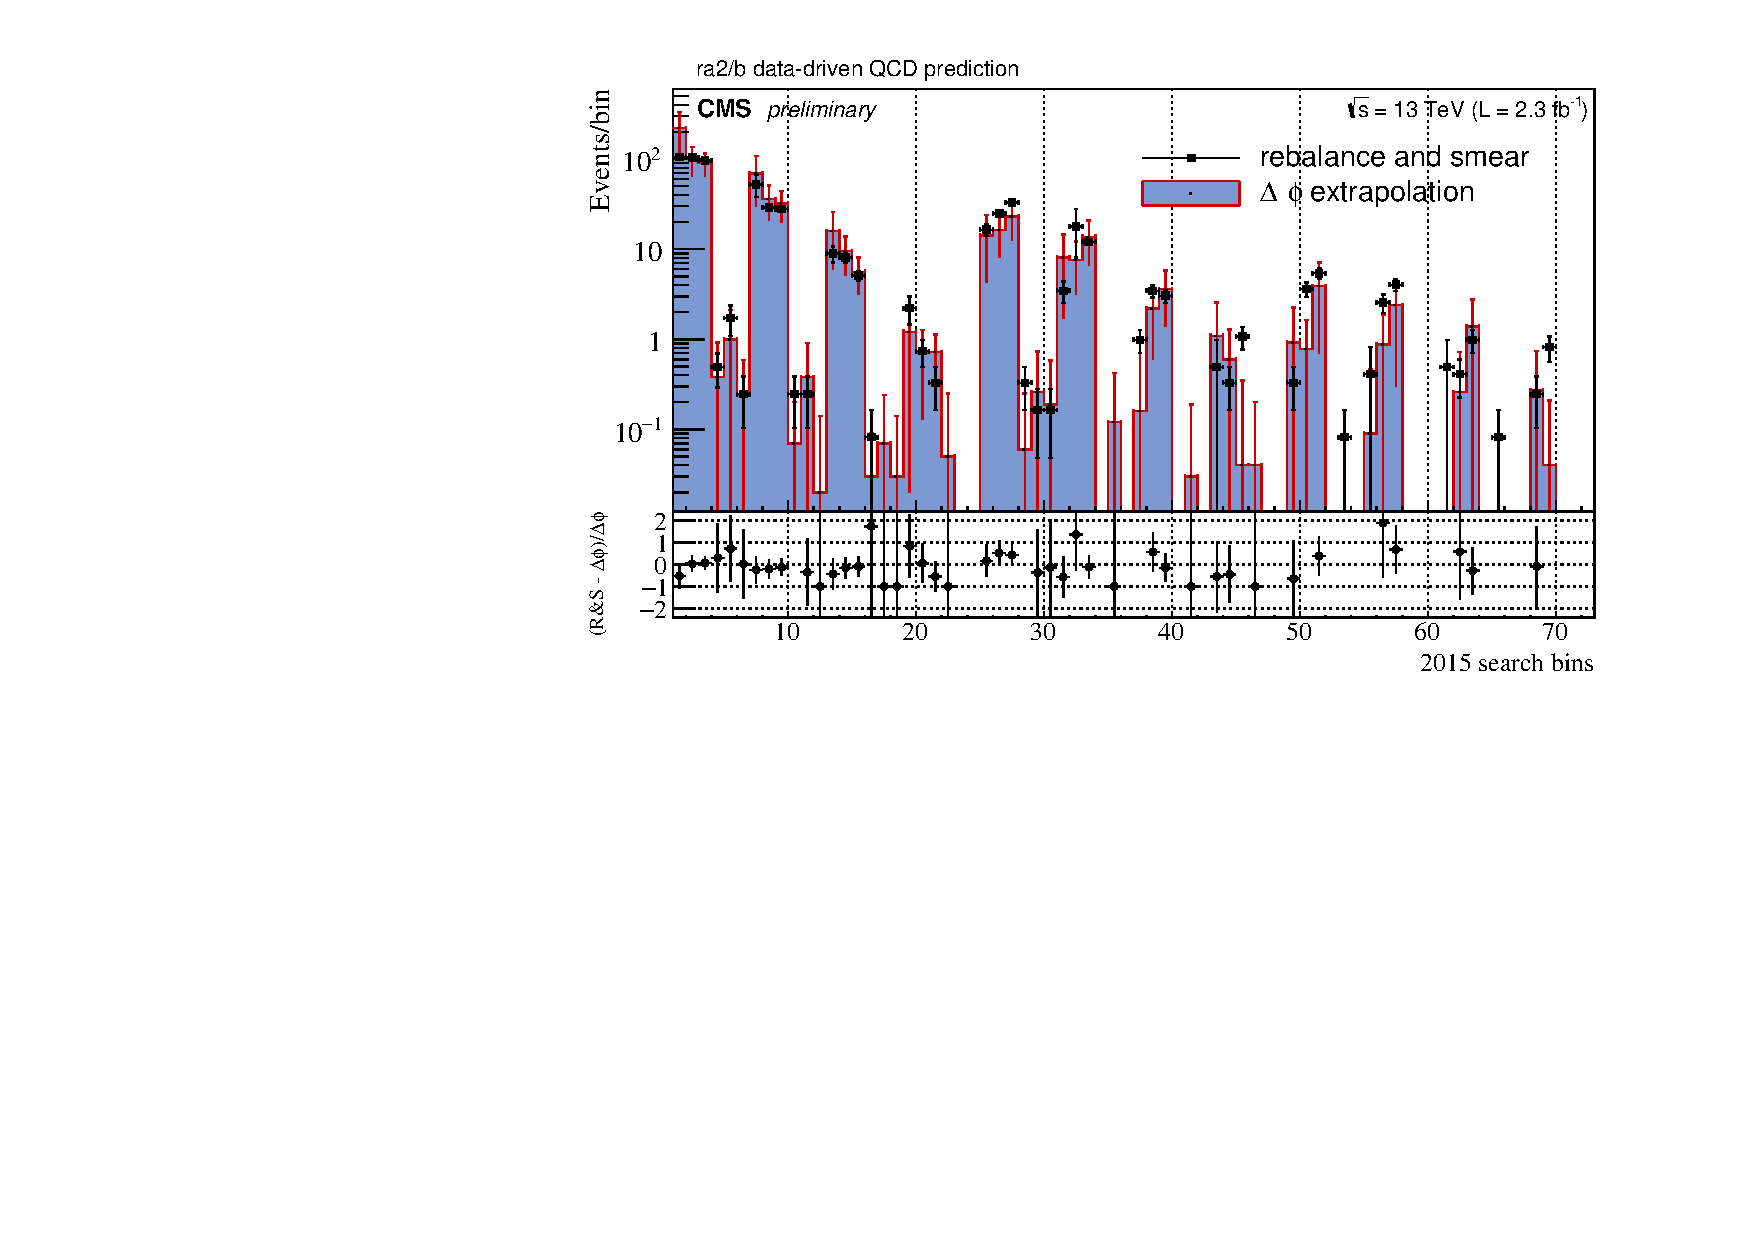
\includegraphics[width=\linewidth]{figures/SusySearches/Ra2b2015/2015CompareQCD.pdf}
\caption{
  The QCD prediction based on the $\Delta\phi$ extrapolation method compared with that of the of rebalance and smear method.}
\label{fig:2015CompareQCD}
\end{figure}



The observed numbers of events in the 72 search regions
are shown in Fig.~\ref{fig:fit-results}
in comparison to the summed predictions for the SM backgrounds,
with numerical values tabulated in Appendix A of~\cite{Khachatryan:2016kdk}. The predicted background is observed to be statistically compatible
with the data for all 72 regions.
Therefore, we do not observe evidence for new physics.
These results are interpreted in the context of the simplified models shown in Fig. \ref{fig:Ra2bSMS}.

\begin{figure}[tb!]
\centering
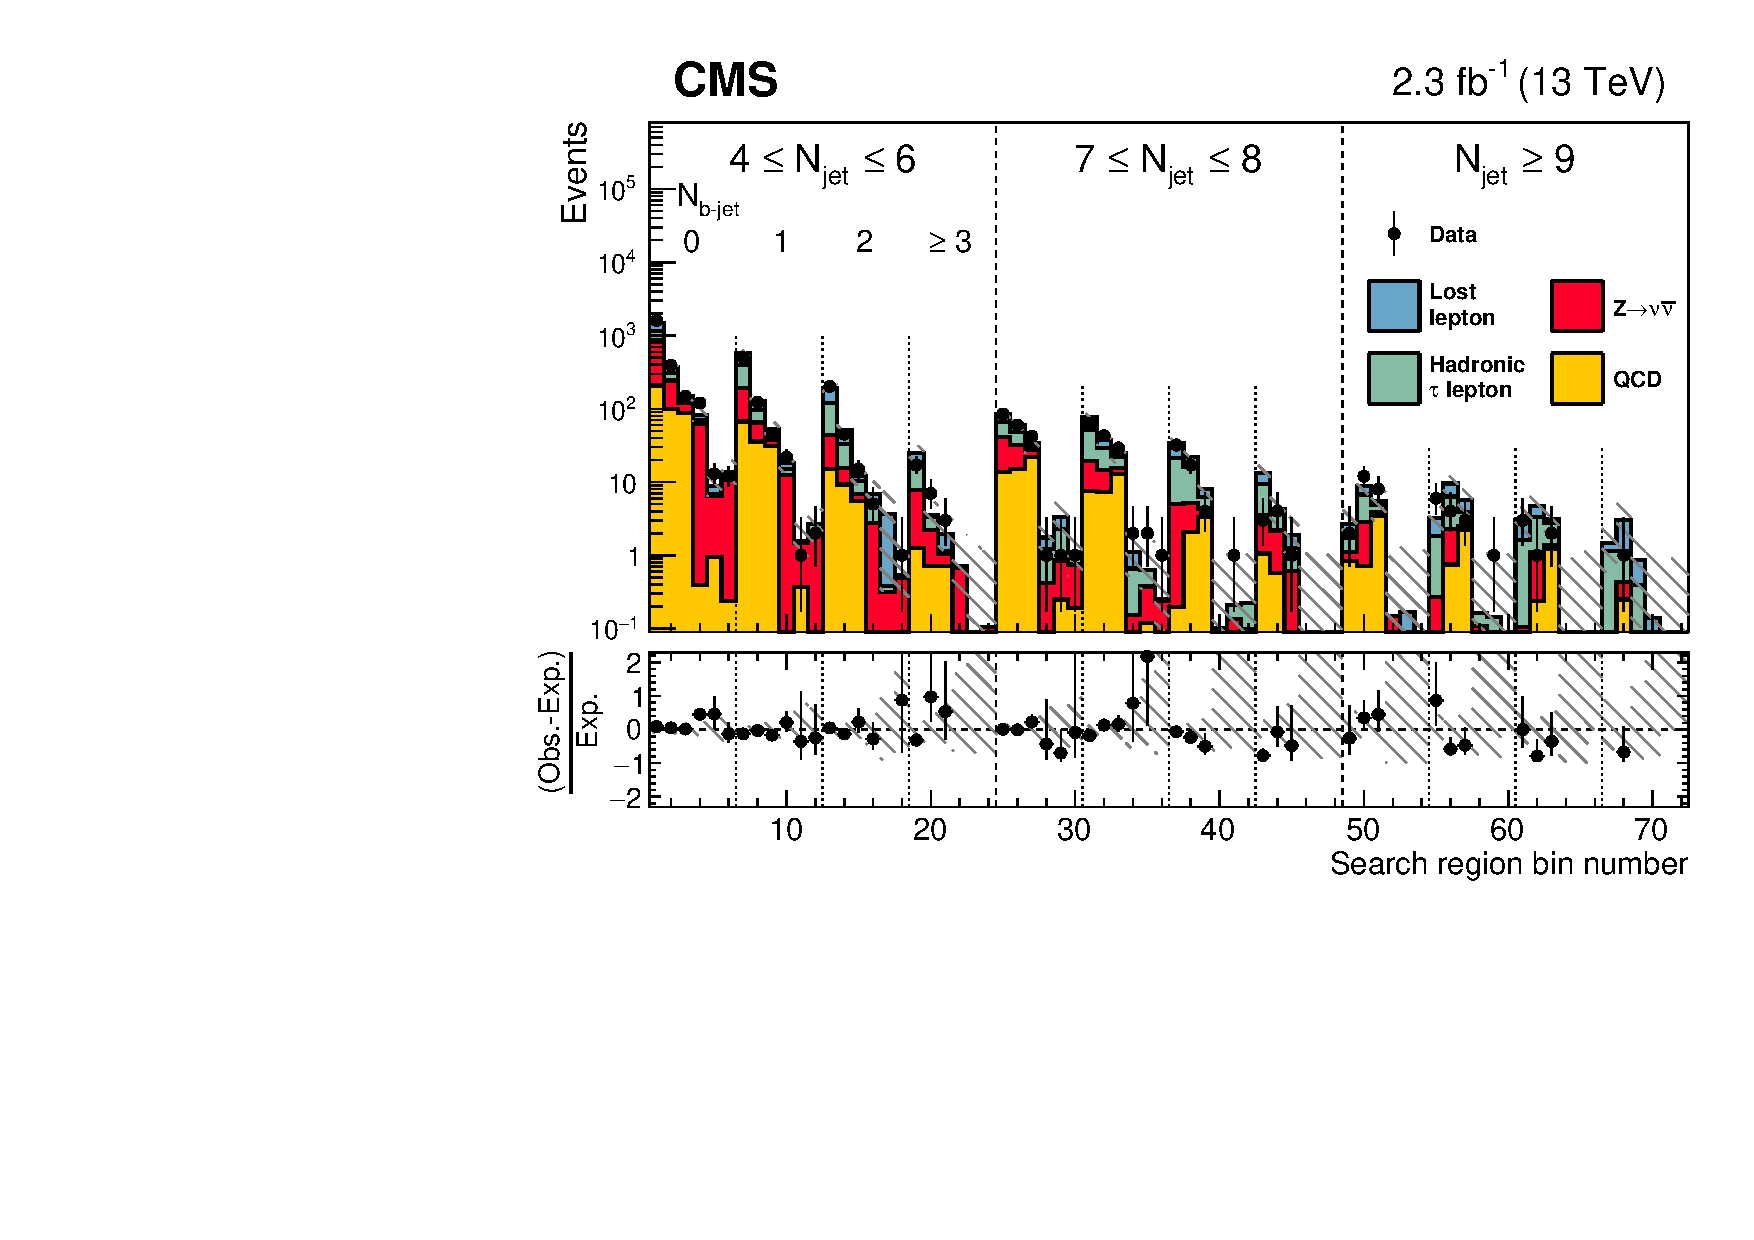
\includegraphics[width=\linewidth]{figures/SusySearches/Ra2b2015/results-plot-prefit.pdf}
\caption{
  Observed numbers of events and corresponding prefit
  SM background predictions
  in the 72 search regions of the analysis,
  with fractional differences shown in the lower panel.
  The shaded regions indicate the total uncertainties in the background
  predictions. For the precise numbering scheme, as well as the final expected and observed counts, please see Appendix \ref{app:anatables}.
}
\label{fig:fit-results}
\end{figure}


For the interpretation, a likelihood fit to data is used to set limits on
the production cross sections of the signal scenarios.
The fitted parameters are the SUSY signal strength,
the yields of the four background classes indicated in Fig.~\ref{fig:fit-results},
and various nuisance parameters.
The limits are determined as a function of $m_{\tilde{\chi}^{0}_{1}}$ and $m_{\tilde{\text{g}}}$.
The likelihood function is the product of Poisson probability functions,
one for each search region,
and constraint terms that account for
uncertainties in the background predictions and signal yields.
These uncertainties are modeled as nuisance parameters
with log-normal probability density functions.
Correlations are taken into account where appropriate.
The signal model uncertainties associated with
the renormalization and factorization scales, ISR,
the jet energy scale,
the b-jet tagging,
and the statistical fluctuations
vary substantially with the event kinematics
and are evaluated as a function of $m_{\tilde{\chi^{0}_{1}}}$ and $m_{\tilde{\text{g}}}$.
The test statistic is
$q_\mu =  - 2 \ln \left( \mathcal{L}_\mu/\mathcal{L}_\text{max} \right)$,
where $\mathcal{L}_\text{max}$ is the maximum likelihood
determined by allowing all parameters including the profile likelihood for the
SUSY signal strength $\mu$ to vary,
and $\mathcal{L}_\mu$ is the maximum likelihood for a fixed signal strength.
To set limits,
we use asymptotic results for the test statistic~\cite{Cowan:2010js}
and the CL$_\mathrm{s}$
method described in Refs.~\cite{Junk1999,bib-cls}. 
Uncertainties in the signal modeling are taken into account when the limits are determined: simulation sample size, luminosity determination ($4.6\%$), lepton and isolated track veto, b-tag efficiency corrections used to scale simulation to data, trigger efficiency, QCD renormalisation and factorization scales, initial/final state radiation (ISR/FSR), signal acceptance and efficiency arising from the jet energy-momentum corrections, jet energy-momentum resolutions, and propagated to \MET, parton distribution functions (PDF) of the proton. More details are provided in Refs.~\cite{cms-note-2011-005,Khachatryan:2015vra}.

\begin{figure*}[htbp]
\centering
    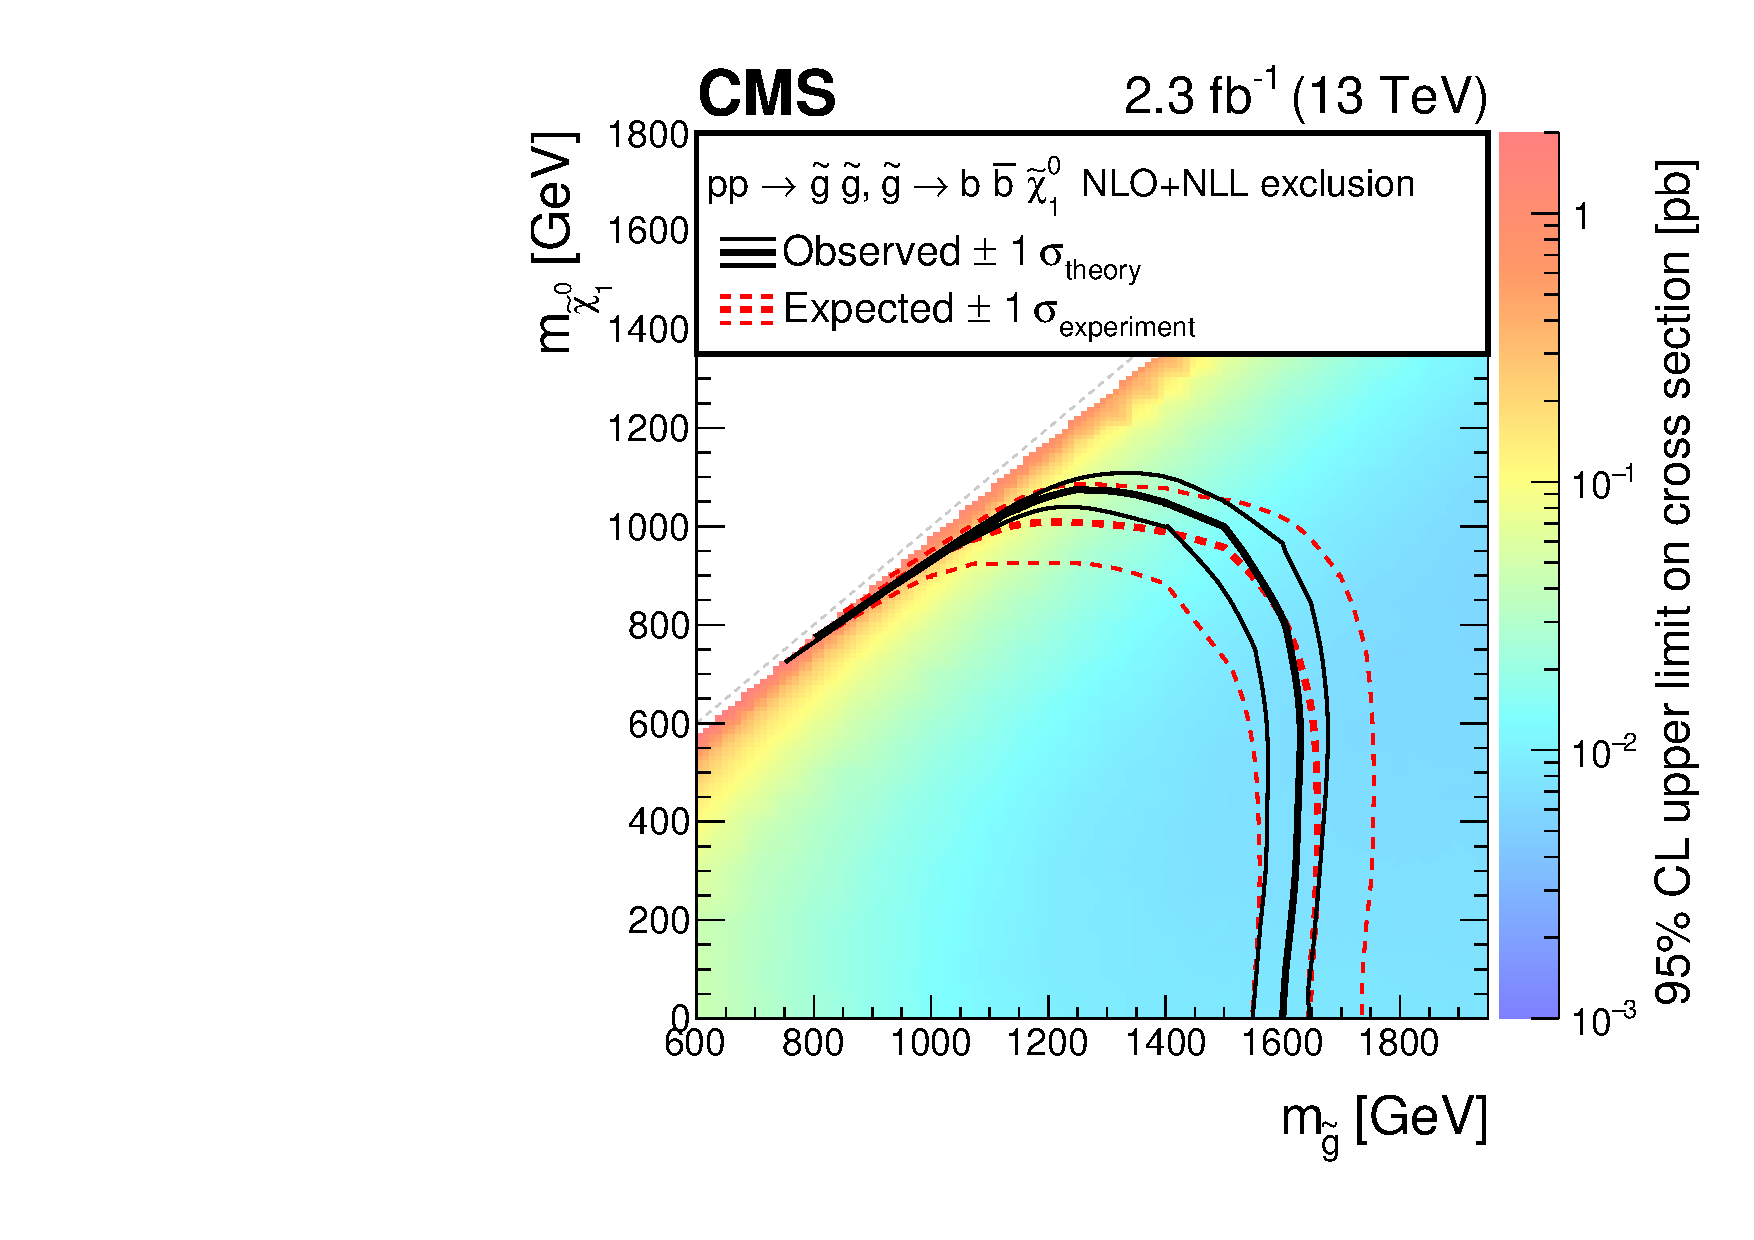
\includegraphics[width=0.48\textwidth]{figures/SusySearches/Ra2b2015/SMSbbbbXSEC.pdf}
    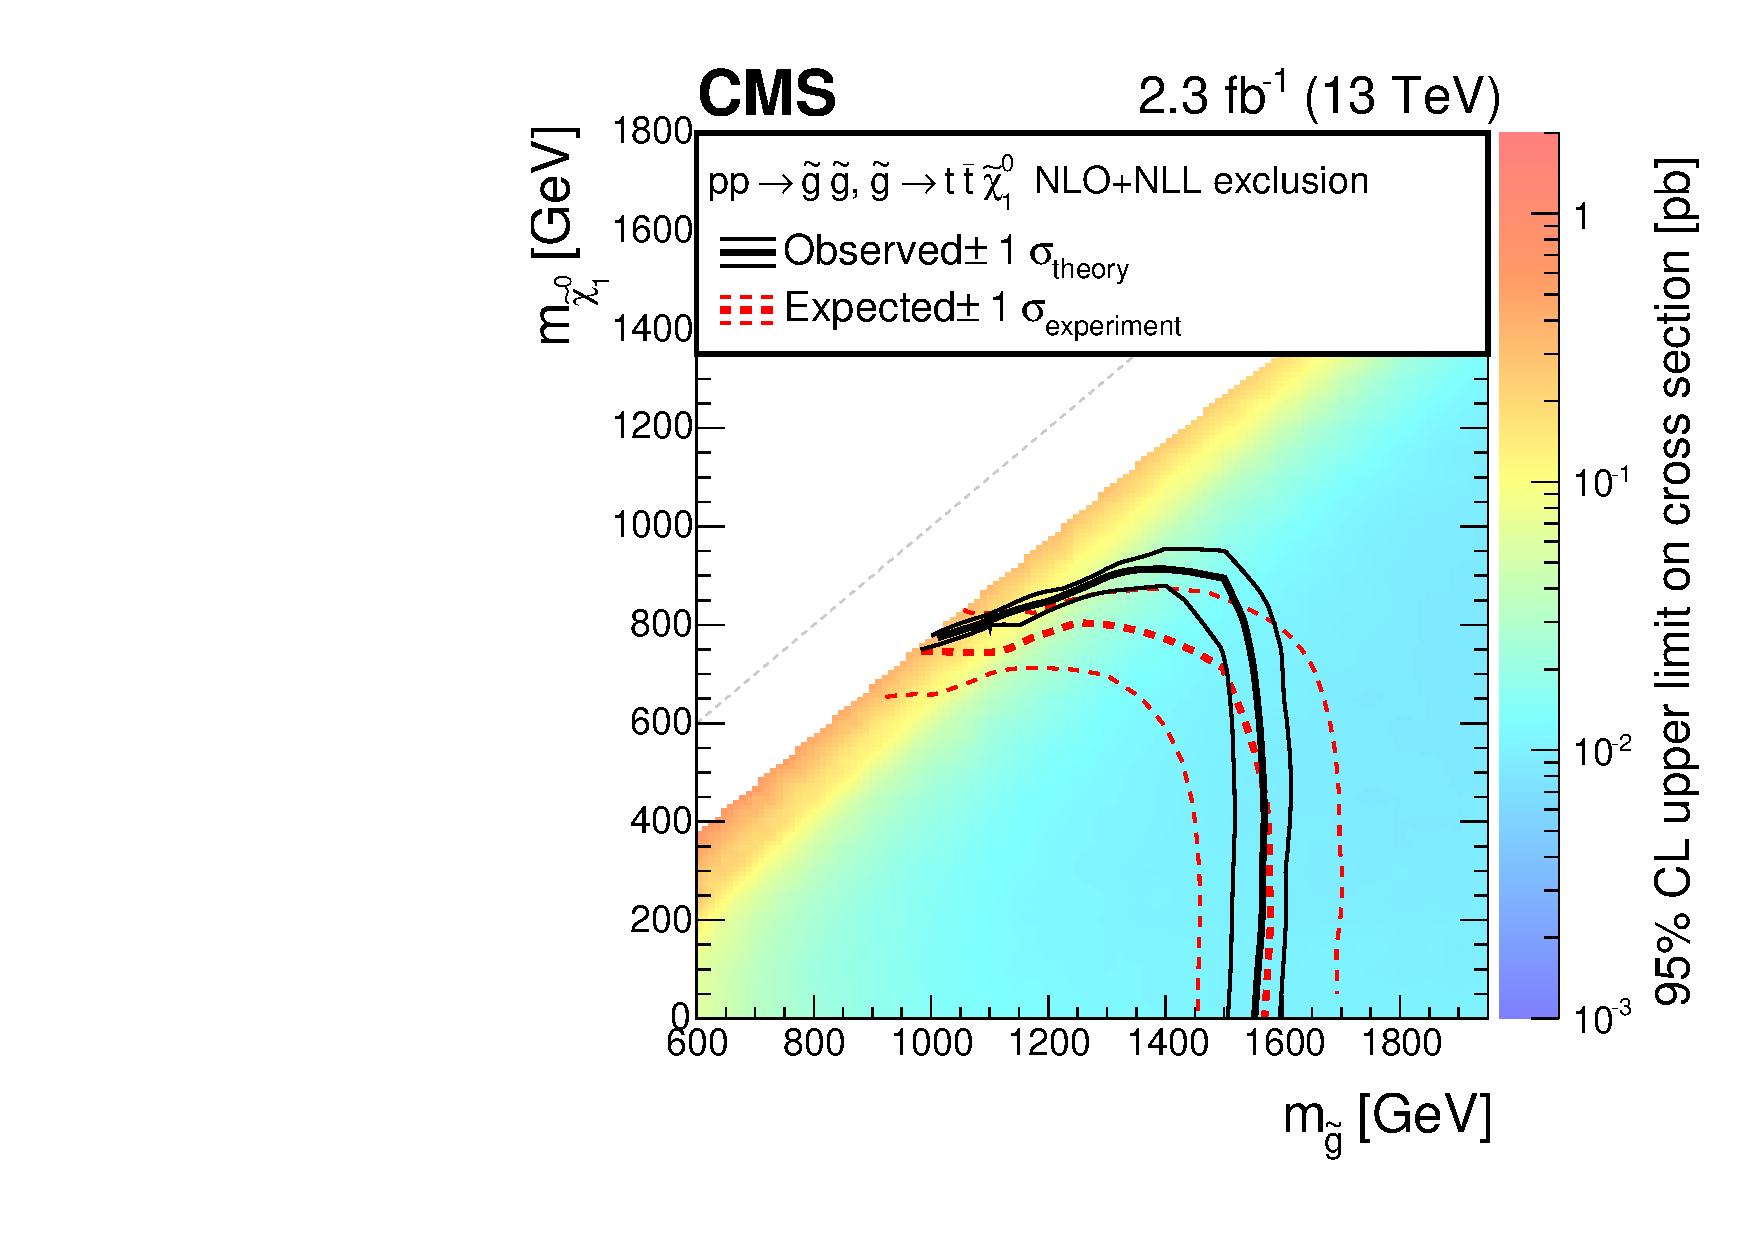
\includegraphics[width=0.48\textwidth]{figures/SusySearches/Ra2b2015/SMSttttXSEC.pdf} \\
    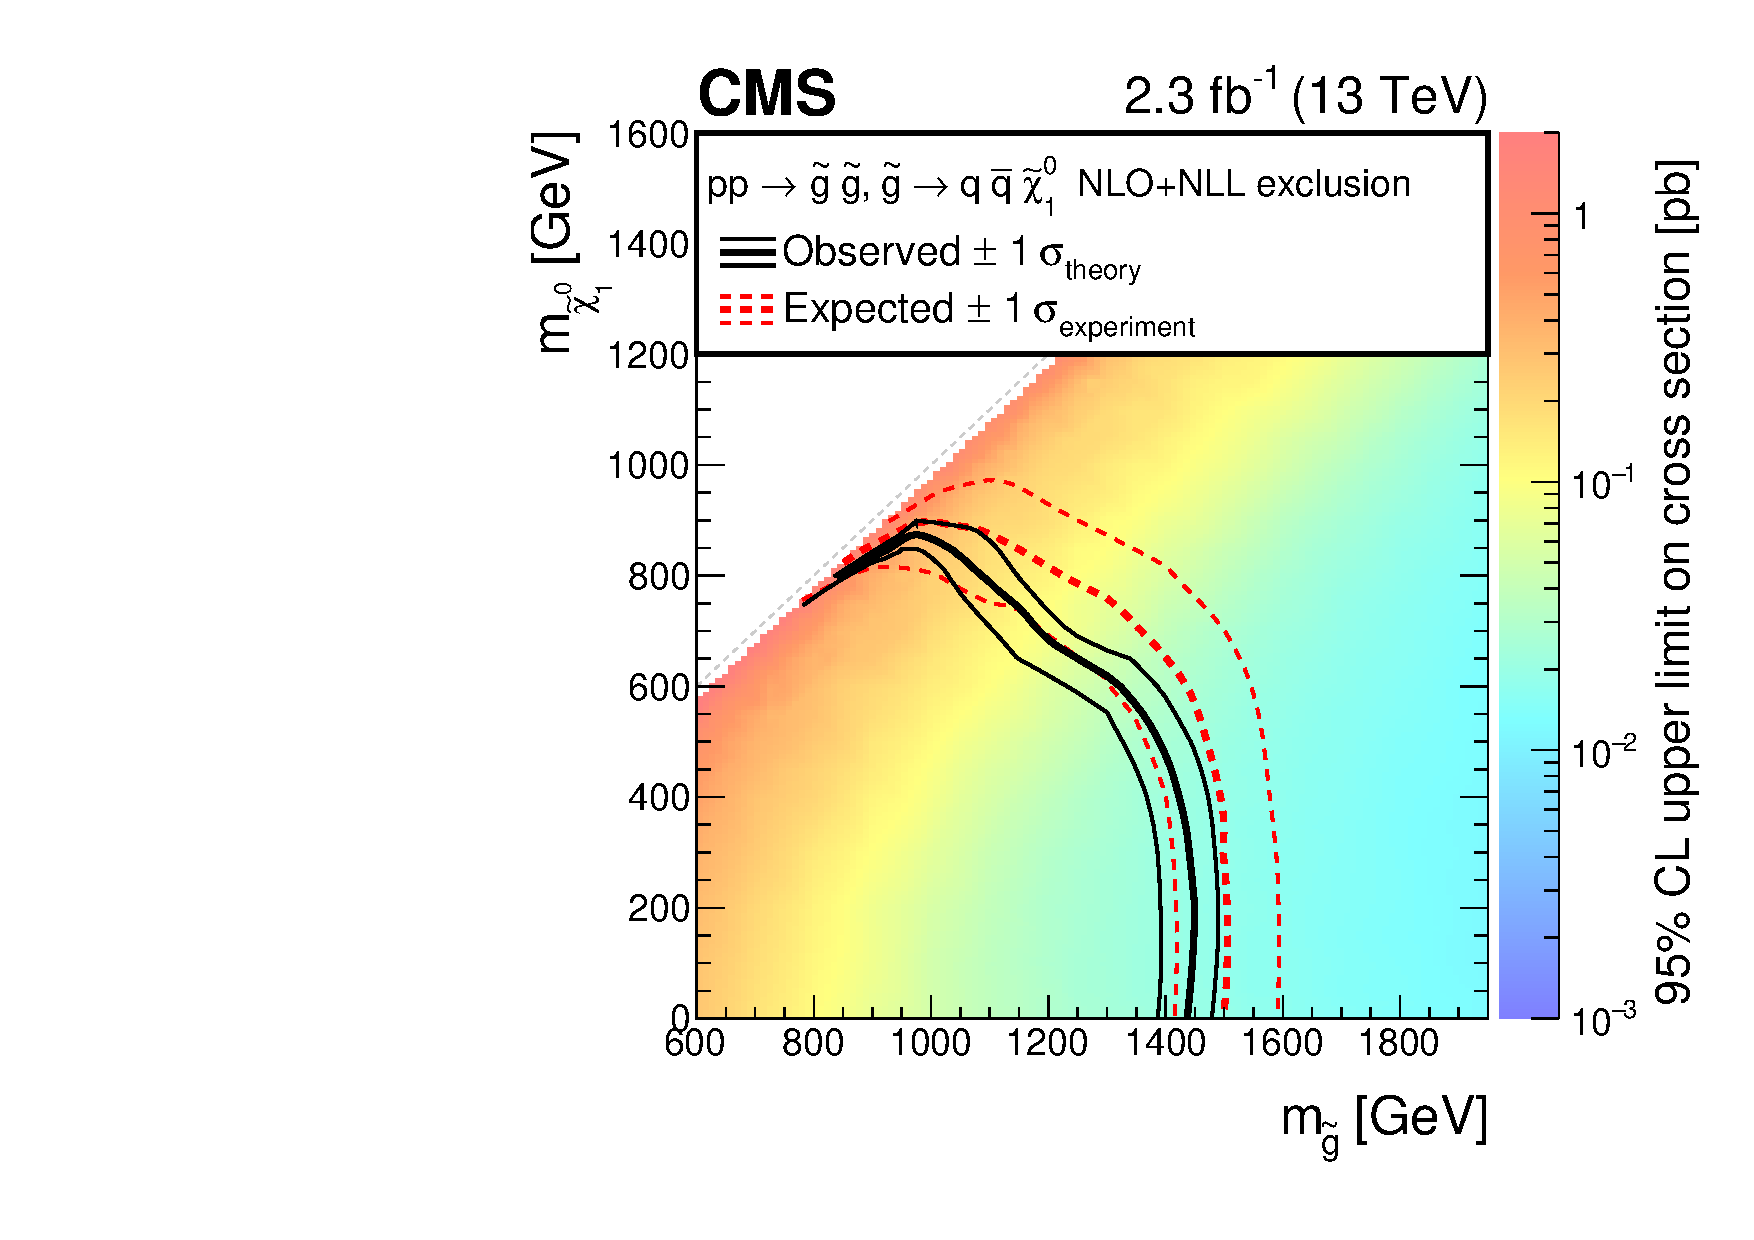
\includegraphics[width=0.48\textwidth]{figures/SusySearches/Ra2b2015/SMSqqqqXSEC.pdf}
    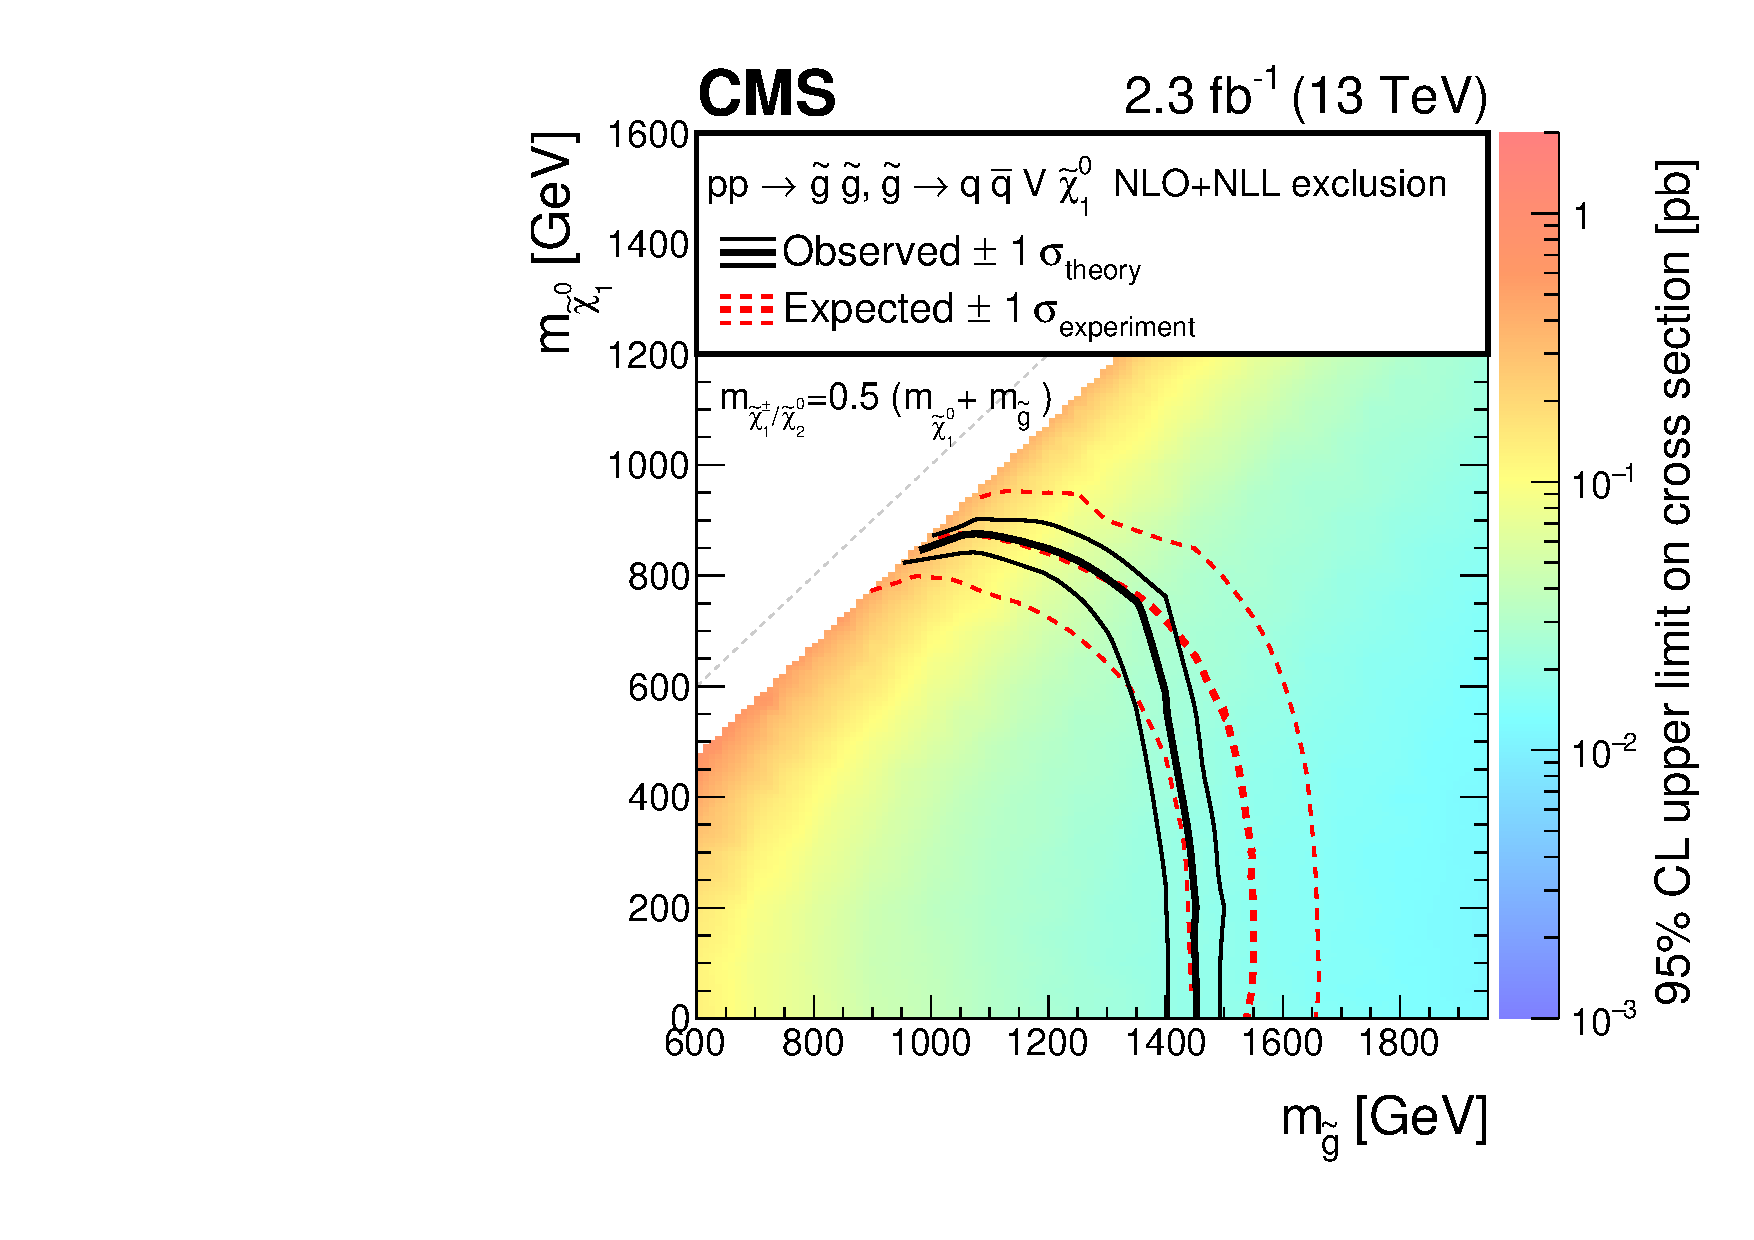
\includegraphics[width=0.48\textwidth]{figures/SusySearches/Ra2b2015/SMSqqqqVVXSEC.pdf}
    \caption{
      The 95\% CL upper limits on the production
      cross sections for the T1bbbb (upper left),
      T1tttt (upper right), T1qqqq (lower left),
      and T5qqqqVV (lower right) simplified models of supersymmetry,
      shown as a function of the gluino and LSP masses $m_{\tilde{\text{g}}}$ and $\tilde{\chi}^{0}_{1}$.
      For the T5qqqqVV model,
      the masses of the intermediate $\tilde{\chi}^{0}_{2}$ and $\tilde{\chi}^{\pm}_{1}$  states
      are taken to be the mean of $m_{\tilde{\chi}^{0}_{1}}$ and $m_{\tilde{\text{g}}}$.
      The solid (black) curves show the observed exclusion contours
      assuming the NLO+NLL cross
      sections, with the corresponding $\pm$1~standard
      deviation uncertainties~\cite{Borschensky:2014cia}.
      The dashed (red) curves are the expected limits
      with $\pm$1 standard deviation experimental uncertainties.
      The dashed (grey) lines indicate the $\tilde{\chi}^{0}_{1}=m_{\tilde{\text{g}}}$ diagonal.
    }
    \label{fig:limits}
\end{figure*}

We proceed to evaluate 95\% confidence level (CL) upper limits
on the signal cross sections.
The NLO+NLL cross section is used as a reference
to evaluate corresponding 95\% CL exclusion curves.
In addition to the observed limits,
expected limits are derived by evaluating the
expected Poisson fluctuations around the predicted
numbers of background events when evaluating the test statistic.
The potential contributions of signal events to the control regions
are taken into account.
Specifically,
the number of events in each CR is corrected
to include the predicted number of signal events,
in the context of the model being examined,
to derive the total effective number of background events
expected in each search region.
This total effective background is used when determining the limits.

The results are shown in Fig.~\ref{fig:limits}. 
For a massless LSP,
we exclude gluinos with masses below 1600, 1550, 1440, and 1450~\GeV,
respectively,
for the T1bbbb, T1tttt, T1qqqq, and T5qqqqVV scenarios. The observed exclusion curves are also shown for the cases in which the signal cross section is varied by changing the renormalization and factorization scales by a factor of 2 and using the PDF4LHC recommendation~\cite{Botje:2011sn} for the PDF uncertainty to illustrate the sensitivity of the exclusion to the signal cross section uncertainty.
These results significantly extend those that were
obtained at $\sqrt{s}=8~\TeV~$,
for which the corresponding limits are around
1150~\GeV~\cite{Chatrchyan:2013wxa,Chatrchyan:2014lfa} for the
three T1 models and 1280~\GeV~\cite{Chatrchyan:2014lfa} for the T5 model.
